% Created by tikzDevice version 0.10.1 on 2016-07-18 19:10:51
% !TEX encoding = UTF-8 Unicode
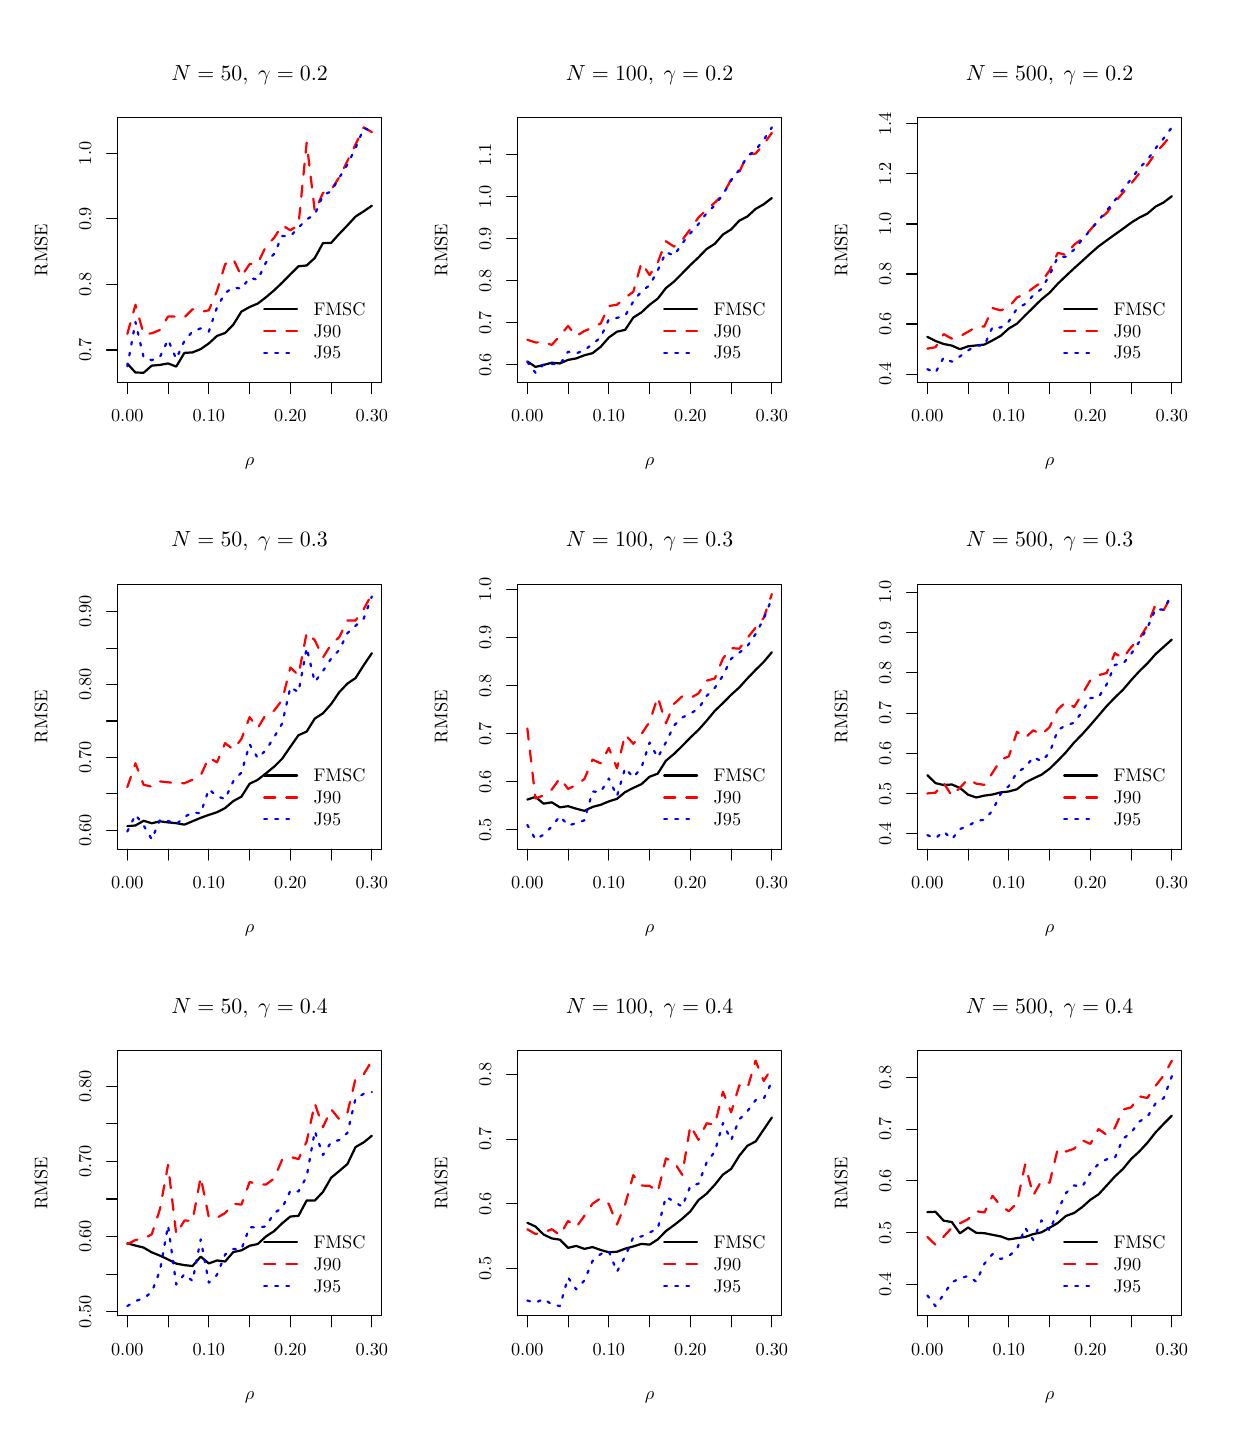
\begin{tikzpicture}[x=1pt,y=1pt]
\definecolor{fillColor}{RGB}{255,255,255}
\path[use as bounding box,fill=fillColor,fill opacity=0.00] (0,0) rectangle (433.62,505.89);
\begin{scope}
\path[clip] ( 32.47,377.65) rectangle (127.91,473.42);
\definecolor{drawColor}{RGB}{0,0,0}

\path[draw=drawColor,line width= 0.8pt,line join=round,line cap=round] ( 36.01,384.47) --
	( 38.95,381.27) --
	( 41.90,381.20) --
	( 44.84,383.76) --
	( 47.79,384.03) --
	( 50.73,384.56) --
	( 53.68,383.42) --
	( 56.63,388.37) --
	( 59.57,388.54) --
	( 62.52,389.75) --
	( 65.46,391.79) --
	( 68.41,394.51) --
	( 71.35,395.56) --
	( 74.30,398.57) --
	( 77.24,403.30) --
	( 80.19,404.94) --
	( 83.14,406.19) --
	( 86.08,408.45) --
	( 89.03,410.95) --
	( 91.97,413.75) --
	( 94.92,416.76) --
	( 97.86,419.67) --
	(100.81,419.96) --
	(103.75,422.66) --
	(106.70,428.01) --
	(109.65,428.12) --
	(112.59,431.38) --
	(115.54,434.44) --
	(118.48,437.64) --
	(121.43,439.53) --
	(124.37,441.54);
\end{scope}
\begin{scope}
\path[clip] (  0.00,  0.00) rectangle (433.62,505.89);
\definecolor{drawColor}{RGB}{0,0,0}

\path[draw=drawColor,line width= 0.4pt,line join=round,line cap=round] ( 36.01,377.65) -- (124.37,377.65);

\path[draw=drawColor,line width= 0.4pt,line join=round,line cap=round] ( 36.01,377.65) -- ( 36.01,373.69);

\path[draw=drawColor,line width= 0.4pt,line join=round,line cap=round] ( 50.73,377.65) -- ( 50.73,373.69);

\path[draw=drawColor,line width= 0.4pt,line join=round,line cap=round] ( 65.46,377.65) -- ( 65.46,373.69);

\path[draw=drawColor,line width= 0.4pt,line join=round,line cap=round] ( 80.19,377.65) -- ( 80.19,373.69);

\path[draw=drawColor,line width= 0.4pt,line join=round,line cap=round] ( 94.92,377.65) -- ( 94.92,373.69);

\path[draw=drawColor,line width= 0.4pt,line join=round,line cap=round] (109.65,377.65) -- (109.65,373.69);

\path[draw=drawColor,line width= 0.4pt,line join=round,line cap=round] (124.37,377.65) -- (124.37,373.69);

\node[text=drawColor,anchor=base,inner sep=0pt, outer sep=0pt, scale=  0.66] at ( 36.01,363.40) {0.00};

\node[text=drawColor,anchor=base,inner sep=0pt, outer sep=0pt, scale=  0.66] at ( 65.46,363.40) {0.10};

\node[text=drawColor,anchor=base,inner sep=0pt, outer sep=0pt, scale=  0.66] at ( 94.92,363.40) {0.20};

\node[text=drawColor,anchor=base,inner sep=0pt, outer sep=0pt, scale=  0.66] at (124.37,363.40) {0.30};

\path[draw=drawColor,line width= 0.4pt,line join=round,line cap=round] ( 32.47,389.43) -- ( 32.47,460.44);

\path[draw=drawColor,line width= 0.4pt,line join=round,line cap=round] ( 32.47,389.43) -- ( 28.51,389.43);

\path[draw=drawColor,line width= 0.4pt,line join=round,line cap=round] ( 32.47,413.10) -- ( 28.51,413.10);

\path[draw=drawColor,line width= 0.4pt,line join=round,line cap=round] ( 32.47,436.77) -- ( 28.51,436.77);

\path[draw=drawColor,line width= 0.4pt,line join=round,line cap=round] ( 32.47,460.44) -- ( 28.51,460.44);

\node[text=drawColor,rotate= 90.00,anchor=base,inner sep=0pt, outer sep=0pt, scale=  0.66] at ( 22.97,389.43) {0.7};

\node[text=drawColor,rotate= 90.00,anchor=base,inner sep=0pt, outer sep=0pt, scale=  0.66] at ( 22.97,413.10) {0.8};

\node[text=drawColor,rotate= 90.00,anchor=base,inner sep=0pt, outer sep=0pt, scale=  0.66] at ( 22.97,436.77) {0.9};

\node[text=drawColor,rotate= 90.00,anchor=base,inner sep=0pt, outer sep=0pt, scale=  0.66] at ( 22.97,460.44) {1.0};

\path[draw=drawColor,line width= 0.4pt,line join=round,line cap=round] ( 32.47,377.65) --
	(127.91,377.65) --
	(127.91,473.42) --
	( 32.47,473.42) --
	( 32.47,377.65);
\end{scope}
\begin{scope}
\path[clip] (  0.00,337.26) rectangle (144.54,505.89);
\definecolor{drawColor}{RGB}{0,0,0}

\node[text=drawColor,anchor=base,inner sep=0pt, outer sep=0pt, scale=  0.79] at ( 80.19,486.92) {\bfseries $N=50, \;\gamma=0.2$};

\node[text=drawColor,anchor=base,inner sep=0pt, outer sep=0pt, scale=  0.66] at ( 80.19,347.56) {$\rho$};

\node[text=drawColor,rotate= 90.00,anchor=base,inner sep=0pt, outer sep=0pt, scale=  0.66] at (  7.13,425.53) {RMSE};
\end{scope}
\begin{scope}
\path[clip] ( 32.47,377.65) rectangle (127.91,473.42);
\definecolor{drawColor}{RGB}{255,0,0}

\path[draw=drawColor,line width= 0.8pt,dash pattern=on 4pt off 4pt ,line join=round,line cap=round] ( 36.01,395.24) --
	( 38.95,405.75) --
	( 41.90,395.19) --
	( 44.84,395.44) --
	( 47.79,396.66) --
	( 50.73,401.50) --
	( 53.68,401.50) --
	( 56.63,401.23) --
	( 59.57,404.14) --
	( 62.52,403.17) --
	( 65.46,403.76) --
	( 68.41,410.76) --
	( 71.35,420.41) --
	( 74.30,422.32) --
	( 77.24,416.02) --
	( 80.19,420.45) --
	( 83.14,420.69) --
	( 86.08,426.85) --
	( 89.03,429.90) --
	( 91.97,434.48) --
	( 94.92,432.66) --
	( 97.86,434.63) --
	(100.81,464.33) --
	(103.75,439.59) --
	(106.70,446.15) --
	(109.65,447.28) --
	(112.59,451.84) --
	(115.54,457.74) --
	(118.48,463.68) --
	(121.43,469.87) --
	(124.37,468.14);
\definecolor{drawColor}{RGB}{0,0,255}

\path[draw=drawColor,line width= 0.8pt,dash pattern=on 1pt off 3pt ,line join=round,line cap=round] ( 36.01,383.52) --
	( 38.95,399.52) --
	( 41.90,386.72) --
	( 44.84,385.72) --
	( 47.79,386.87) --
	( 50.73,393.13) --
	( 53.68,386.20) --
	( 56.63,392.69) --
	( 59.57,396.13) --
	( 62.52,397.22) --
	( 65.46,396.07) --
	( 68.41,404.79) --
	( 71.35,410.03) --
	( 74.30,412.02) --
	( 77.24,411.57) --
	( 80.19,415.52) --
	( 83.14,414.80) --
	( 86.08,421.03) --
	( 89.03,424.13) --
	( 91.97,430.57) --
	( 94.92,430.54) --
	( 97.86,433.60) --
	(100.81,436.63) --
	(103.75,438.32) --
	(106.70,445.34) --
	(109.65,446.73) --
	(112.59,451.63) --
	(115.54,456.45) --
	(118.48,462.39) --
	(121.43,469.56) --
	(124.37,468.54);
\definecolor{drawColor}{RGB}{0,0,0}

\path[draw=drawColor,line width= 0.8pt,line join=round,line cap=round] ( 85.47,404.28) -- ( 97.35,404.28);
\definecolor{drawColor}{RGB}{255,0,0}

\path[draw=drawColor,line width= 0.8pt,dash pattern=on 4pt off 4pt ,line join=round,line cap=round] ( 85.47,396.36) -- ( 97.35,396.36);
\definecolor{drawColor}{RGB}{0,0,255}

\path[draw=drawColor,line width= 0.8pt,dash pattern=on 1pt off 3pt ,line join=round,line cap=round] ( 85.47,388.44) -- ( 97.35,388.44);
\definecolor{drawColor}{RGB}{0,0,0}

\node[text=drawColor,anchor=base west,inner sep=0pt, outer sep=0pt, scale=  0.66] at (103.29,402.01) {FMSC};

\node[text=drawColor,anchor=base west,inner sep=0pt, outer sep=0pt, scale=  0.66] at (103.29,394.09) {J90};

\node[text=drawColor,anchor=base west,inner sep=0pt, outer sep=0pt, scale=  0.66] at (103.29,386.17) {J95};
\end{scope}
\begin{scope}
\path[clip] (177.01,377.65) rectangle (272.45,473.42);
\definecolor{drawColor}{RGB}{0,0,0}

\path[draw=drawColor,line width= 0.8pt,line join=round,line cap=round] (180.55,385.30) --
	(183.49,383.30) --
	(186.44,384.02) --
	(189.38,384.81) --
	(192.33,384.56) --
	(195.27,385.84) --
	(198.22,386.37) --
	(201.17,387.51) --
	(204.11,388.27) --
	(207.06,390.57) --
	(210.00,393.93) --
	(212.95,396.03) --
	(215.89,396.70) --
	(218.84,401.14) --
	(221.78,403.00) --
	(224.73,405.76) --
	(227.68,407.96) --
	(230.62,411.78) --
	(233.57,414.15) --
	(236.51,417.10) --
	(239.46,420.11) --
	(242.40,422.89) --
	(245.35,425.92) --
	(248.29,427.78) --
	(251.24,431.15) --
	(254.19,432.98) --
	(257.13,436.14) --
	(260.08,437.67) --
	(263.02,440.37) --
	(265.97,442.08) --
	(268.91,444.33);
\end{scope}
\begin{scope}
\path[clip] (  0.00,  0.00) rectangle (433.62,505.89);
\definecolor{drawColor}{RGB}{0,0,0}

\path[draw=drawColor,line width= 0.4pt,line join=round,line cap=round] (180.55,377.65) -- (268.91,377.65);

\path[draw=drawColor,line width= 0.4pt,line join=round,line cap=round] (180.55,377.65) -- (180.55,373.69);

\path[draw=drawColor,line width= 0.4pt,line join=round,line cap=round] (195.27,377.65) -- (195.27,373.69);

\path[draw=drawColor,line width= 0.4pt,line join=round,line cap=round] (210.00,377.65) -- (210.00,373.69);

\path[draw=drawColor,line width= 0.4pt,line join=round,line cap=round] (224.73,377.65) -- (224.73,373.69);

\path[draw=drawColor,line width= 0.4pt,line join=round,line cap=round] (239.46,377.65) -- (239.46,373.69);

\path[draw=drawColor,line width= 0.4pt,line join=round,line cap=round] (254.19,377.65) -- (254.19,373.69);

\path[draw=drawColor,line width= 0.4pt,line join=round,line cap=round] (268.91,377.65) -- (268.91,373.69);

\node[text=drawColor,anchor=base,inner sep=0pt, outer sep=0pt, scale=  0.66] at (180.55,363.40) {0.00};

\node[text=drawColor,anchor=base,inner sep=0pt, outer sep=0pt, scale=  0.66] at (210.00,363.40) {0.10};

\node[text=drawColor,anchor=base,inner sep=0pt, outer sep=0pt, scale=  0.66] at (239.46,363.40) {0.20};

\node[text=drawColor,anchor=base,inner sep=0pt, outer sep=0pt, scale=  0.66] at (268.91,363.40) {0.30};

\path[draw=drawColor,line width= 0.4pt,line join=round,line cap=round] (177.01,384.08) -- (177.01,459.98);

\path[draw=drawColor,line width= 0.4pt,line join=round,line cap=round] (177.01,384.08) -- (173.05,384.08);

\path[draw=drawColor,line width= 0.4pt,line join=round,line cap=round] (177.01,399.26) -- (173.05,399.26);

\path[draw=drawColor,line width= 0.4pt,line join=round,line cap=round] (177.01,414.44) -- (173.05,414.44);

\path[draw=drawColor,line width= 0.4pt,line join=round,line cap=round] (177.01,429.62) -- (173.05,429.62);

\path[draw=drawColor,line width= 0.4pt,line join=round,line cap=round] (177.01,444.80) -- (173.05,444.80);

\path[draw=drawColor,line width= 0.4pt,line join=round,line cap=round] (177.01,459.98) -- (173.05,459.98);

\node[text=drawColor,rotate= 90.00,anchor=base,inner sep=0pt, outer sep=0pt, scale=  0.66] at (167.51,384.08) {0.6};

\node[text=drawColor,rotate= 90.00,anchor=base,inner sep=0pt, outer sep=0pt, scale=  0.66] at (167.51,399.26) {0.7};

\node[text=drawColor,rotate= 90.00,anchor=base,inner sep=0pt, outer sep=0pt, scale=  0.66] at (167.51,414.44) {0.8};

\node[text=drawColor,rotate= 90.00,anchor=base,inner sep=0pt, outer sep=0pt, scale=  0.66] at (167.51,429.62) {0.9};

\node[text=drawColor,rotate= 90.00,anchor=base,inner sep=0pt, outer sep=0pt, scale=  0.66] at (167.51,444.80) {1.0};

\node[text=drawColor,rotate= 90.00,anchor=base,inner sep=0pt, outer sep=0pt, scale=  0.66] at (167.51,459.98) {1.1};

\path[draw=drawColor,line width= 0.4pt,line join=round,line cap=round] (177.01,377.65) --
	(272.45,377.65) --
	(272.45,473.42) --
	(177.01,473.42) --
	(177.01,377.65);
\end{scope}
\begin{scope}
\path[clip] (144.54,337.26) rectangle (289.08,505.89);
\definecolor{drawColor}{RGB}{0,0,0}

\node[text=drawColor,anchor=base,inner sep=0pt, outer sep=0pt, scale=  0.79] at (224.73,486.92) {\bfseries $N=100, \;\gamma=0.2$};

\node[text=drawColor,anchor=base,inner sep=0pt, outer sep=0pt, scale=  0.66] at (224.73,347.56) {$\rho$};

\node[text=drawColor,rotate= 90.00,anchor=base,inner sep=0pt, outer sep=0pt, scale=  0.66] at (151.67,425.53) {RMSE};
\end{scope}
\begin{scope}
\path[clip] (177.01,377.65) rectangle (272.45,473.42);
\definecolor{drawColor}{RGB}{255,0,0}

\path[draw=drawColor,line width= 0.8pt,dash pattern=on 4pt off 4pt ,line join=round,line cap=round] (180.55,393.10) --
	(183.49,392.15) --
	(186.44,392.20) --
	(189.38,391.25) --
	(192.33,394.59) --
	(195.27,398.08) --
	(198.22,394.42) --
	(201.17,396.30) --
	(204.11,397.45) --
	(207.06,399.00) --
	(210.00,405.31) --
	(212.95,405.77) --
	(215.89,408.27) --
	(218.84,410.46) --
	(221.78,420.93) --
	(224.73,416.50) --
	(227.68,421.08) --
	(230.62,428.71) --
	(233.57,426.77) --
	(236.51,429.13) --
	(239.46,433.12) --
	(242.40,437.31) --
	(245.35,440.11) --
	(248.29,442.67) --
	(251.24,445.52) --
	(254.19,451.04) --
	(257.13,453.68) --
	(260.08,460.16) --
	(263.02,460.38) --
	(265.97,463.79) --
	(268.91,467.89);
\definecolor{drawColor}{RGB}{0,0,255}

\path[draw=drawColor,line width= 0.8pt,dash pattern=on 1pt off 3pt ,line join=round,line cap=round] (180.55,385.10) --
	(183.49,381.20) --
	(186.44,384.20) --
	(189.38,384.38) --
	(192.33,384.16) --
	(195.27,388.80) --
	(198.22,388.16) --
	(201.17,389.37) --
	(204.11,391.55) --
	(207.06,393.98) --
	(210.00,400.49) --
	(212.95,401.03) --
	(215.89,401.77) --
	(218.84,406.95) --
	(221.78,410.60) --
	(224.73,412.79) --
	(227.68,418.17) --
	(230.62,424.74) --
	(233.57,423.56) --
	(236.51,427.93) --
	(239.46,431.61) --
	(242.40,434.92) --
	(245.35,438.90) --
	(248.29,441.70) --
	(251.24,445.59) --
	(254.19,450.71) --
	(257.13,454.53) --
	(260.08,459.42) --
	(263.02,461.66) --
	(265.97,465.35) --
	(268.91,469.87);
\definecolor{drawColor}{RGB}{0,0,0}

\path[draw=drawColor,line width= 0.8pt,line join=round,line cap=round] (230.01,404.28) -- (241.89,404.28);
\definecolor{drawColor}{RGB}{255,0,0}

\path[draw=drawColor,line width= 0.8pt,dash pattern=on 4pt off 4pt ,line join=round,line cap=round] (230.01,396.36) -- (241.89,396.36);
\definecolor{drawColor}{RGB}{0,0,255}

\path[draw=drawColor,line width= 0.8pt,dash pattern=on 1pt off 3pt ,line join=round,line cap=round] (230.01,388.44) -- (241.89,388.44);
\definecolor{drawColor}{RGB}{0,0,0}

\node[text=drawColor,anchor=base west,inner sep=0pt, outer sep=0pt, scale=  0.66] at (247.83,402.01) {FMSC};

\node[text=drawColor,anchor=base west,inner sep=0pt, outer sep=0pt, scale=  0.66] at (247.83,394.09) {J90};

\node[text=drawColor,anchor=base west,inner sep=0pt, outer sep=0pt, scale=  0.66] at (247.83,386.17) {J95};
\end{scope}
\begin{scope}
\path[clip] (321.55,377.65) rectangle (416.99,473.42);
\definecolor{drawColor}{RGB}{0,0,0}

\path[draw=drawColor,line width= 0.8pt,line join=round,line cap=round] (325.09,394.17) --
	(328.03,392.67) --
	(330.98,391.59) --
	(333.92,391.02) --
	(336.87,389.70) --
	(339.81,390.73) --
	(342.76,391.06) --
	(345.71,391.38) --
	(348.65,392.89) --
	(351.60,394.54) --
	(354.54,397.18) --
	(357.49,398.93) --
	(360.43,401.91) --
	(363.38,404.78) --
	(366.32,407.70) --
	(369.27,410.10) --
	(372.22,413.35) --
	(375.16,416.16) --
	(378.11,418.92) --
	(381.05,421.57) --
	(384.00,424.27) --
	(386.94,426.85) --
	(389.89,429.01) --
	(392.83,431.13) --
	(395.78,433.22) --
	(398.73,435.40) --
	(401.67,437.25) --
	(404.62,438.69) --
	(407.56,441.23) --
	(410.51,442.75) --
	(413.45,444.99);
\end{scope}
\begin{scope}
\path[clip] (  0.00,  0.00) rectangle (433.62,505.89);
\definecolor{drawColor}{RGB}{0,0,0}

\path[draw=drawColor,line width= 0.4pt,line join=round,line cap=round] (325.09,377.65) -- (413.45,377.65);

\path[draw=drawColor,line width= 0.4pt,line join=round,line cap=round] (325.09,377.65) -- (325.09,373.69);

\path[draw=drawColor,line width= 0.4pt,line join=round,line cap=round] (339.81,377.65) -- (339.81,373.69);

\path[draw=drawColor,line width= 0.4pt,line join=round,line cap=round] (354.54,377.65) -- (354.54,373.69);

\path[draw=drawColor,line width= 0.4pt,line join=round,line cap=round] (369.27,377.65) -- (369.27,373.69);

\path[draw=drawColor,line width= 0.4pt,line join=round,line cap=round] (384.00,377.65) -- (384.00,373.69);

\path[draw=drawColor,line width= 0.4pt,line join=round,line cap=round] (398.73,377.65) -- (398.73,373.69);

\path[draw=drawColor,line width= 0.4pt,line join=round,line cap=round] (413.45,377.65) -- (413.45,373.69);

\node[text=drawColor,anchor=base,inner sep=0pt, outer sep=0pt, scale=  0.66] at (325.09,363.40) {0.00};

\node[text=drawColor,anchor=base,inner sep=0pt, outer sep=0pt, scale=  0.66] at (354.54,363.40) {0.10};

\node[text=drawColor,anchor=base,inner sep=0pt, outer sep=0pt, scale=  0.66] at (384.00,363.40) {0.20};

\node[text=drawColor,anchor=base,inner sep=0pt, outer sep=0pt, scale=  0.66] at (413.45,363.40) {0.30};

\path[draw=drawColor,line width= 0.4pt,line join=round,line cap=round] (321.55,380.72) -- (321.55,471.11);

\path[draw=drawColor,line width= 0.4pt,line join=round,line cap=round] (321.55,380.72) -- (317.59,380.72);

\path[draw=drawColor,line width= 0.4pt,line join=round,line cap=round] (321.55,398.80) -- (317.59,398.80);

\path[draw=drawColor,line width= 0.4pt,line join=round,line cap=round] (321.55,416.87) -- (317.59,416.87);

\path[draw=drawColor,line width= 0.4pt,line join=round,line cap=round] (321.55,434.95) -- (317.59,434.95);

\path[draw=drawColor,line width= 0.4pt,line join=round,line cap=round] (321.55,453.03) -- (317.59,453.03);

\path[draw=drawColor,line width= 0.4pt,line join=round,line cap=round] (321.55,471.11) -- (317.59,471.11);

\node[text=drawColor,rotate= 90.00,anchor=base,inner sep=0pt, outer sep=0pt, scale=  0.66] at (312.05,380.72) {0.4};

\node[text=drawColor,rotate= 90.00,anchor=base,inner sep=0pt, outer sep=0pt, scale=  0.66] at (312.05,398.80) {0.6};

\node[text=drawColor,rotate= 90.00,anchor=base,inner sep=0pt, outer sep=0pt, scale=  0.66] at (312.05,416.87) {0.8};

\node[text=drawColor,rotate= 90.00,anchor=base,inner sep=0pt, outer sep=0pt, scale=  0.66] at (312.05,434.95) {1.0};

\node[text=drawColor,rotate= 90.00,anchor=base,inner sep=0pt, outer sep=0pt, scale=  0.66] at (312.05,453.03) {1.2};

\node[text=drawColor,rotate= 90.00,anchor=base,inner sep=0pt, outer sep=0pt, scale=  0.66] at (312.05,471.11) {1.4};

\path[draw=drawColor,line width= 0.4pt,line join=round,line cap=round] (321.55,377.65) --
	(416.99,377.65) --
	(416.99,473.42) --
	(321.55,473.42) --
	(321.55,377.65);
\end{scope}
\begin{scope}
\path[clip] (289.08,337.26) rectangle (433.62,505.89);
\definecolor{drawColor}{RGB}{0,0,0}

\node[text=drawColor,anchor=base,inner sep=0pt, outer sep=0pt, scale=  0.79] at (369.27,486.92) {\bfseries $N=500, \;\gamma=0.2$};

\node[text=drawColor,anchor=base,inner sep=0pt, outer sep=0pt, scale=  0.66] at (369.27,347.56) {$\rho$};

\node[text=drawColor,rotate= 90.00,anchor=base,inner sep=0pt, outer sep=0pt, scale=  0.66] at (296.21,425.53) {RMSE};
\end{scope}
\begin{scope}
\path[clip] (321.55,377.65) rectangle (416.99,473.42);
\definecolor{drawColor}{RGB}{255,0,0}

\path[draw=drawColor,line width= 0.8pt,dash pattern=on 4pt off 4pt ,line join=round,line cap=round] (325.09,389.91) --
	(328.03,390.42) --
	(330.98,395.15) --
	(333.92,393.53) --
	(336.87,394.34) --
	(339.81,396.01) --
	(342.76,397.76) --
	(345.71,397.93) --
	(348.65,404.58) --
	(351.60,403.72) --
	(354.54,404.88) --
	(357.49,408.42) --
	(360.43,409.58) --
	(363.38,411.87) --
	(366.32,413.92) --
	(369.27,418.22) --
	(372.22,424.51) --
	(375.16,423.78) --
	(378.11,427.44) --
	(381.05,429.63) --
	(384.00,432.85) --
	(386.94,436.31) --
	(389.89,438.95) --
	(392.83,442.76) --
	(395.78,446.27) --
	(398.73,449.50) --
	(401.67,453.27) --
	(404.62,456.33) --
	(407.56,460.54) --
	(410.51,463.85) --
	(413.45,467.46);
\definecolor{drawColor}{RGB}{0,0,255}

\path[draw=drawColor,line width= 0.8pt,dash pattern=on 1pt off 3pt ,line join=round,line cap=round] (325.09,382.49) --
	(328.03,381.20) --
	(330.98,386.69) --
	(333.92,385.16) --
	(336.87,387.10) --
	(339.81,389.25) --
	(342.76,391.00) --
	(345.71,391.11) --
	(348.65,397.73) --
	(351.60,397.51) --
	(354.54,399.77) --
	(357.49,404.43) --
	(360.43,406.03) --
	(363.38,409.21) --
	(366.32,411.49) --
	(369.27,416.50) --
	(372.22,423.00) --
	(375.16,423.11) --
	(378.11,425.69) --
	(381.05,429.34) --
	(384.00,432.71) --
	(386.94,436.24) --
	(389.89,439.76) --
	(392.83,443.47) --
	(395.78,447.47) --
	(398.73,451.19) --
	(401.67,455.13) --
	(404.62,458.08) --
	(407.56,462.29) --
	(410.51,465.92) --
	(413.45,469.87);
\definecolor{drawColor}{RGB}{0,0,0}

\path[draw=drawColor,line width= 0.8pt,line join=round,line cap=round] (374.55,404.28) -- (386.43,404.28);
\definecolor{drawColor}{RGB}{255,0,0}

\path[draw=drawColor,line width= 0.8pt,dash pattern=on 4pt off 4pt ,line join=round,line cap=round] (374.55,396.36) -- (386.43,396.36);
\definecolor{drawColor}{RGB}{0,0,255}

\path[draw=drawColor,line width= 0.8pt,dash pattern=on 1pt off 3pt ,line join=round,line cap=round] (374.55,388.44) -- (386.43,388.44);
\definecolor{drawColor}{RGB}{0,0,0}

\node[text=drawColor,anchor=base west,inner sep=0pt, outer sep=0pt, scale=  0.66] at (392.37,402.01) {FMSC};

\node[text=drawColor,anchor=base west,inner sep=0pt, outer sep=0pt, scale=  0.66] at (392.37,394.09) {J90};

\node[text=drawColor,anchor=base west,inner sep=0pt, outer sep=0pt, scale=  0.66] at (392.37,386.17) {J95};
\end{scope}
\begin{scope}
\path[clip] ( 32.47,209.02) rectangle (127.91,304.79);
\definecolor{drawColor}{RGB}{0,0,0}

\path[draw=drawColor,line width= 0.8pt,line join=round,line cap=round] ( 36.01,217.36) --
	( 38.95,217.60) --
	( 41.90,219.31) --
	( 44.84,218.40) --
	( 47.79,219.10) --
	( 50.73,218.71) --
	( 53.68,218.43) --
	( 56.63,217.90) --
	( 59.57,219.13) --
	( 62.52,220.36) --
	( 65.46,221.43) --
	( 68.41,222.38) --
	( 71.35,223.90) --
	( 74.30,226.42) --
	( 77.24,228.01) --
	( 80.19,232.68) --
	( 83.14,234.10) --
	( 86.08,236.42) --
	( 89.03,238.82) --
	( 91.97,241.74) --
	( 94.92,246.04) --
	( 97.86,250.23) --
	(100.81,251.53) --
	(103.75,256.24) --
	(106.70,258.13) --
	(109.65,261.46) --
	(112.59,265.77) --
	(115.54,268.88) --
	(118.48,270.86) --
	(121.43,275.53) --
	(124.37,279.86);
\end{scope}
\begin{scope}
\path[clip] (  0.00,  0.00) rectangle (433.62,505.89);
\definecolor{drawColor}{RGB}{0,0,0}

\path[draw=drawColor,line width= 0.4pt,line join=round,line cap=round] ( 36.01,209.02) -- (124.37,209.02);

\path[draw=drawColor,line width= 0.4pt,line join=round,line cap=round] ( 36.01,209.02) -- ( 36.01,205.06);

\path[draw=drawColor,line width= 0.4pt,line join=round,line cap=round] ( 50.73,209.02) -- ( 50.73,205.06);

\path[draw=drawColor,line width= 0.4pt,line join=round,line cap=round] ( 65.46,209.02) -- ( 65.46,205.06);

\path[draw=drawColor,line width= 0.4pt,line join=round,line cap=round] ( 80.19,209.02) -- ( 80.19,205.06);

\path[draw=drawColor,line width= 0.4pt,line join=round,line cap=round] ( 94.92,209.02) -- ( 94.92,205.06);

\path[draw=drawColor,line width= 0.4pt,line join=round,line cap=round] (109.65,209.02) -- (109.65,205.06);

\path[draw=drawColor,line width= 0.4pt,line join=round,line cap=round] (124.37,209.02) -- (124.37,205.06);

\node[text=drawColor,anchor=base,inner sep=0pt, outer sep=0pt, scale=  0.66] at ( 36.01,194.77) {0.00};

\node[text=drawColor,anchor=base,inner sep=0pt, outer sep=0pt, scale=  0.66] at ( 65.46,194.77) {0.10};

\node[text=drawColor,anchor=base,inner sep=0pt, outer sep=0pt, scale=  0.66] at ( 94.92,194.77) {0.20};

\node[text=drawColor,anchor=base,inner sep=0pt, outer sep=0pt, scale=  0.66] at (124.37,194.77) {0.30};

\path[draw=drawColor,line width= 0.4pt,line join=round,line cap=round] ( 32.47,215.87) -- ( 32.47,294.83);

\path[draw=drawColor,line width= 0.4pt,line join=round,line cap=round] ( 32.47,215.87) -- ( 28.51,215.87);

\path[draw=drawColor,line width= 0.4pt,line join=round,line cap=round] ( 32.47,229.03) -- ( 28.51,229.03);

\path[draw=drawColor,line width= 0.4pt,line join=round,line cap=round] ( 32.47,242.19) -- ( 28.51,242.19);

\path[draw=drawColor,line width= 0.4pt,line join=round,line cap=round] ( 32.47,255.35) -- ( 28.51,255.35);

\path[draw=drawColor,line width= 0.4pt,line join=round,line cap=round] ( 32.47,268.51) -- ( 28.51,268.51);

\path[draw=drawColor,line width= 0.4pt,line join=round,line cap=round] ( 32.47,281.67) -- ( 28.51,281.67);

\path[draw=drawColor,line width= 0.4pt,line join=round,line cap=round] ( 32.47,294.83) -- ( 28.51,294.83);

\node[text=drawColor,rotate= 90.00,anchor=base,inner sep=0pt, outer sep=0pt, scale=  0.66] at ( 22.97,215.87) {0.60};

\node[text=drawColor,rotate= 90.00,anchor=base,inner sep=0pt, outer sep=0pt, scale=  0.66] at ( 22.97,242.19) {0.70};

\node[text=drawColor,rotate= 90.00,anchor=base,inner sep=0pt, outer sep=0pt, scale=  0.66] at ( 22.97,268.51) {0.80};

\node[text=drawColor,rotate= 90.00,anchor=base,inner sep=0pt, outer sep=0pt, scale=  0.66] at ( 22.97,294.83) {0.90};

\path[draw=drawColor,line width= 0.4pt,line join=round,line cap=round] ( 32.47,209.02) --
	(127.91,209.02) --
	(127.91,304.79) --
	( 32.47,304.79) --
	( 32.47,209.02);
\end{scope}
\begin{scope}
\path[clip] (  0.00,168.63) rectangle (144.54,337.26);
\definecolor{drawColor}{RGB}{0,0,0}

\node[text=drawColor,anchor=base,inner sep=0pt, outer sep=0pt, scale=  0.79] at ( 80.19,318.29) {\bfseries $N=50, \;\gamma=0.3$};

\node[text=drawColor,anchor=base,inner sep=0pt, outer sep=0pt, scale=  0.66] at ( 80.19,178.93) {$\rho$};

\node[text=drawColor,rotate= 90.00,anchor=base,inner sep=0pt, outer sep=0pt, scale=  0.66] at (  7.13,256.90) {RMSE};
\end{scope}
\begin{scope}
\path[clip] ( 32.47,209.02) rectangle (127.91,304.79);
\definecolor{drawColor}{RGB}{255,0,0}

\path[draw=drawColor,line width= 0.8pt,dash pattern=on 4pt off 4pt ,line join=round,line cap=round] ( 36.01,231.44) --
	( 38.95,240.07) --
	( 41.90,232.31) --
	( 44.84,231.61) --
	( 47.79,233.52) --
	( 50.73,233.20) --
	( 53.68,232.90) --
	( 56.63,232.88) --
	( 59.57,234.14) --
	( 62.52,235.71) --
	( 65.46,242.11) --
	( 68.41,240.43) --
	( 71.35,247.37) --
	( 74.30,245.03) --
	( 77.24,248.88) --
	( 80.19,256.74) --
	( 83.14,252.80) --
	( 86.08,257.72) --
	( 89.03,259.11) --
	( 91.97,262.92) --
	( 94.92,274.69) --
	( 97.86,271.89) --
	(100.81,287.25) --
	(103.75,284.56) --
	(106.70,278.29) --
	(109.65,283.02) --
	(112.59,285.65) --
	(115.54,291.69) --
	(118.48,291.67) --
	(121.43,295.77) --
	(124.37,301.24);
\definecolor{drawColor}{RGB}{0,0,255}

\path[draw=drawColor,line width= 0.8pt,dash pattern=on 1pt off 3pt ,line join=round,line cap=round] ( 36.01,215.40) --
	( 38.95,221.51) --
	( 41.90,217.65) --
	( 44.84,212.57) --
	( 47.79,219.59) --
	( 50.73,219.25) --
	( 53.68,218.00) --
	( 56.63,220.68) --
	( 59.57,222.33) --
	( 62.52,221.99) --
	( 65.46,230.73) --
	( 68.41,228.13) --
	( 71.35,227.19) --
	( 74.30,233.59) --
	( 77.24,236.75) --
	( 80.19,246.94) --
	( 83.14,241.94) --
	( 86.08,244.85) --
	( 89.03,249.48) --
	( 91.97,254.46) --
	( 94.92,267.54) --
	( 97.86,265.78) --
	(100.81,281.80) --
	(103.75,269.45) --
	(106.70,273.41) --
	(109.65,277.89) --
	(112.59,281.00) --
	(115.54,287.11) --
	(118.48,289.75) --
	(121.43,292.37) --
	(124.37,300.36);
\definecolor{drawColor}{RGB}{0,0,0}

\path[draw=drawColor,line width= 0.8pt,line join=round,line cap=round] ( 85.47,235.65) -- ( 97.35,235.65);
\definecolor{drawColor}{RGB}{255,0,0}

\path[draw=drawColor,line width= 0.8pt,dash pattern=on 4pt off 4pt ,line join=round,line cap=round] ( 85.47,227.73) -- ( 97.35,227.73);
\definecolor{drawColor}{RGB}{0,0,255}

\path[draw=drawColor,line width= 0.8pt,dash pattern=on 1pt off 3pt ,line join=round,line cap=round] ( 85.47,219.81) -- ( 97.35,219.81);
\definecolor{drawColor}{RGB}{0,0,0}

\node[text=drawColor,anchor=base west,inner sep=0pt, outer sep=0pt, scale=  0.66] at (103.29,233.38) {FMSC};

\node[text=drawColor,anchor=base west,inner sep=0pt, outer sep=0pt, scale=  0.66] at (103.29,225.46) {J90};

\node[text=drawColor,anchor=base west,inner sep=0pt, outer sep=0pt, scale=  0.66] at (103.29,217.54) {J95};
\end{scope}
\begin{scope}
\path[clip] (177.01,209.02) rectangle (272.45,304.79);
\definecolor{drawColor}{RGB}{0,0,0}

\path[draw=drawColor,line width= 0.8pt,line join=round,line cap=round] (180.55,226.97) --
	(183.49,227.91) --
	(186.44,225.48) --
	(189.38,225.97) --
	(192.33,224.15) --
	(195.27,224.57) --
	(198.22,223.66) --
	(201.17,222.90) --
	(204.11,224.31) --
	(207.06,225.07) --
	(210.00,226.30) --
	(212.95,227.24) --
	(215.89,229.66) --
	(218.84,231.18) --
	(221.78,232.52) --
	(224.73,235.21) --
	(227.68,236.33) --
	(230.62,240.99) --
	(233.57,243.47) --
	(236.51,246.33) --
	(239.46,249.37) --
	(242.40,252.15) --
	(245.35,255.46) --
	(248.29,259.02) --
	(251.24,261.83) --
	(254.19,264.83) --
	(257.13,267.47) --
	(260.08,270.74) --
	(263.02,273.79) --
	(265.97,276.70) --
	(268.91,280.20);
\end{scope}
\begin{scope}
\path[clip] (  0.00,  0.00) rectangle (433.62,505.89);
\definecolor{drawColor}{RGB}{0,0,0}

\path[draw=drawColor,line width= 0.4pt,line join=round,line cap=round] (180.55,209.02) -- (268.91,209.02);

\path[draw=drawColor,line width= 0.4pt,line join=round,line cap=round] (180.55,209.02) -- (180.55,205.06);

\path[draw=drawColor,line width= 0.4pt,line join=round,line cap=round] (195.27,209.02) -- (195.27,205.06);

\path[draw=drawColor,line width= 0.4pt,line join=round,line cap=round] (210.00,209.02) -- (210.00,205.06);

\path[draw=drawColor,line width= 0.4pt,line join=round,line cap=round] (224.73,209.02) -- (224.73,205.06);

\path[draw=drawColor,line width= 0.4pt,line join=round,line cap=round] (239.46,209.02) -- (239.46,205.06);

\path[draw=drawColor,line width= 0.4pt,line join=round,line cap=round] (254.19,209.02) -- (254.19,205.06);

\path[draw=drawColor,line width= 0.4pt,line join=round,line cap=round] (268.91,209.02) -- (268.91,205.06);

\node[text=drawColor,anchor=base,inner sep=0pt, outer sep=0pt, scale=  0.66] at (180.55,194.77) {0.00};

\node[text=drawColor,anchor=base,inner sep=0pt, outer sep=0pt, scale=  0.66] at (210.00,194.77) {0.10};

\node[text=drawColor,anchor=base,inner sep=0pt, outer sep=0pt, scale=  0.66] at (239.46,194.77) {0.20};

\node[text=drawColor,anchor=base,inner sep=0pt, outer sep=0pt, scale=  0.66] at (268.91,194.77) {0.30};

\path[draw=drawColor,line width= 0.4pt,line join=round,line cap=round] (177.01,216.02) -- (177.01,302.92);

\path[draw=drawColor,line width= 0.4pt,line join=round,line cap=round] (177.01,216.02) -- (173.05,216.02);

\path[draw=drawColor,line width= 0.4pt,line join=round,line cap=round] (177.01,233.40) -- (173.05,233.40);

\path[draw=drawColor,line width= 0.4pt,line join=round,line cap=round] (177.01,250.78) -- (173.05,250.78);

\path[draw=drawColor,line width= 0.4pt,line join=round,line cap=round] (177.01,268.16) -- (173.05,268.16);

\path[draw=drawColor,line width= 0.4pt,line join=round,line cap=round] (177.01,285.54) -- (173.05,285.54);

\path[draw=drawColor,line width= 0.4pt,line join=round,line cap=round] (177.01,302.92) -- (173.05,302.92);

\node[text=drawColor,rotate= 90.00,anchor=base,inner sep=0pt, outer sep=0pt, scale=  0.66] at (167.51,216.02) {0.5};

\node[text=drawColor,rotate= 90.00,anchor=base,inner sep=0pt, outer sep=0pt, scale=  0.66] at (167.51,233.40) {0.6};

\node[text=drawColor,rotate= 90.00,anchor=base,inner sep=0pt, outer sep=0pt, scale=  0.66] at (167.51,250.78) {0.7};

\node[text=drawColor,rotate= 90.00,anchor=base,inner sep=0pt, outer sep=0pt, scale=  0.66] at (167.51,268.16) {0.8};

\node[text=drawColor,rotate= 90.00,anchor=base,inner sep=0pt, outer sep=0pt, scale=  0.66] at (167.51,285.54) {0.9};

\node[text=drawColor,rotate= 90.00,anchor=base,inner sep=0pt, outer sep=0pt, scale=  0.66] at (167.51,302.92) {1.0};

\path[draw=drawColor,line width= 0.4pt,line join=round,line cap=round] (177.01,209.02) --
	(272.45,209.02) --
	(272.45,304.79) --
	(177.01,304.79) --
	(177.01,209.02);
\end{scope}
\begin{scope}
\path[clip] (144.54,168.63) rectangle (289.08,337.26);
\definecolor{drawColor}{RGB}{0,0,0}

\node[text=drawColor,anchor=base,inner sep=0pt, outer sep=0pt, scale=  0.79] at (224.73,318.29) {\bfseries $N=100, \;\gamma=0.3$};

\node[text=drawColor,anchor=base,inner sep=0pt, outer sep=0pt, scale=  0.66] at (224.73,178.93) {$\rho$};

\node[text=drawColor,rotate= 90.00,anchor=base,inner sep=0pt, outer sep=0pt, scale=  0.66] at (151.67,256.90) {RMSE};
\end{scope}
\begin{scope}
\path[clip] (177.01,209.02) rectangle (272.45,304.79);
\definecolor{drawColor}{RGB}{255,0,0}

\path[draw=drawColor,line width= 0.8pt,dash pattern=on 4pt off 4pt ,line join=round,line cap=round] (180.55,252.62) --
	(183.49,227.36) --
	(186.44,228.50) --
	(189.38,230.60) --
	(192.33,234.68) --
	(195.27,230.80) --
	(198.22,232.18) --
	(201.17,234.39) --
	(204.11,241.39) --
	(207.06,240.05) --
	(210.00,245.61) --
	(212.95,238.25) --
	(215.89,250.44) --
	(218.84,247.12) --
	(221.78,250.67) --
	(224.73,255.06) --
	(227.68,264.03) --
	(230.62,254.49) --
	(233.57,261.56) --
	(236.51,264.27) --
	(239.46,263.64) --
	(242.40,265.33) --
	(245.35,269.93) --
	(248.29,270.71) --
	(251.24,277.95) --
	(254.19,281.71) --
	(257.13,281.48) --
	(260.08,285.40) --
	(263.02,289.06) --
	(265.97,292.64) --
	(268.91,301.24);
\definecolor{drawColor}{RGB}{0,0,255}

\path[draw=drawColor,line width= 0.8pt,dash pattern=on 1pt off 3pt ,line join=round,line cap=round] (180.55,217.80) --
	(183.49,212.57) --
	(186.44,214.28) --
	(189.38,217.27) --
	(192.33,220.97) --
	(195.27,217.62) --
	(198.22,218.39) --
	(201.17,219.49) --
	(204.11,229.87) --
	(207.06,229.70) --
	(210.00,234.59) --
	(212.95,228.21) --
	(215.89,238.35) --
	(218.84,234.98) --
	(221.78,238.49) --
	(224.73,247.56) --
	(227.68,242.16) --
	(230.62,247.66) --
	(233.57,253.74) --
	(236.51,256.61) --
	(239.46,258.01) --
	(242.40,259.83) --
	(245.35,264.42) --
	(248.29,267.34) --
	(251.24,271.76) --
	(254.19,277.86) --
	(257.13,280.02) --
	(260.08,282.43) --
	(263.02,286.75) --
	(265.97,292.30) --
	(268.91,299.65);
\definecolor{drawColor}{RGB}{0,0,0}

\path[draw=drawColor,line width= 0.8pt,line join=round,line cap=round] (230.01,235.65) -- (241.89,235.65);
\definecolor{drawColor}{RGB}{255,0,0}

\path[draw=drawColor,line width= 0.8pt,dash pattern=on 4pt off 4pt ,line join=round,line cap=round] (230.01,227.73) -- (241.89,227.73);
\definecolor{drawColor}{RGB}{0,0,255}

\path[draw=drawColor,line width= 0.8pt,dash pattern=on 1pt off 3pt ,line join=round,line cap=round] (230.01,219.81) -- (241.89,219.81);
\definecolor{drawColor}{RGB}{0,0,0}

\node[text=drawColor,anchor=base west,inner sep=0pt, outer sep=0pt, scale=  0.66] at (247.83,233.38) {FMSC};

\node[text=drawColor,anchor=base west,inner sep=0pt, outer sep=0pt, scale=  0.66] at (247.83,225.46) {J90};

\node[text=drawColor,anchor=base west,inner sep=0pt, outer sep=0pt, scale=  0.66] at (247.83,217.54) {J95};
\end{scope}
\begin{scope}
\path[clip] (321.55,209.02) rectangle (416.99,304.79);
\definecolor{drawColor}{RGB}{0,0,0}

\path[draw=drawColor,line width= 0.8pt,line join=round,line cap=round] (325.09,235.82) --
	(328.03,232.90) --
	(330.98,232.21) --
	(333.92,232.41) --
	(336.87,231.18) --
	(339.81,228.72) --
	(342.76,227.72) --
	(345.71,228.39) --
	(348.65,228.80) --
	(351.60,229.56) --
	(354.54,229.89) --
	(357.49,230.70) --
	(360.43,233.05) --
	(363.38,234.58) --
	(366.32,235.93) --
	(369.27,238.11) --
	(372.22,240.97) --
	(375.16,244.04) --
	(378.11,247.56) --
	(381.05,250.56) --
	(384.00,253.85) --
	(386.94,257.28) --
	(389.89,260.74) --
	(392.83,263.79) --
	(395.78,266.63) --
	(398.73,270.10) --
	(401.67,273.31) --
	(404.62,276.17) --
	(407.56,279.52) --
	(410.51,282.16) --
	(413.45,284.79);
\end{scope}
\begin{scope}
\path[clip] (  0.00,  0.00) rectangle (433.62,505.89);
\definecolor{drawColor}{RGB}{0,0,0}

\path[draw=drawColor,line width= 0.4pt,line join=round,line cap=round] (325.09,209.02) -- (413.45,209.02);

\path[draw=drawColor,line width= 0.4pt,line join=round,line cap=round] (325.09,209.02) -- (325.09,205.06);

\path[draw=drawColor,line width= 0.4pt,line join=round,line cap=round] (339.81,209.02) -- (339.81,205.06);

\path[draw=drawColor,line width= 0.4pt,line join=round,line cap=round] (354.54,209.02) -- (354.54,205.06);

\path[draw=drawColor,line width= 0.4pt,line join=round,line cap=round] (369.27,209.02) -- (369.27,205.06);

\path[draw=drawColor,line width= 0.4pt,line join=round,line cap=round] (384.00,209.02) -- (384.00,205.06);

\path[draw=drawColor,line width= 0.4pt,line join=round,line cap=round] (398.73,209.02) -- (398.73,205.06);

\path[draw=drawColor,line width= 0.4pt,line join=round,line cap=round] (413.45,209.02) -- (413.45,205.06);

\node[text=drawColor,anchor=base,inner sep=0pt, outer sep=0pt, scale=  0.66] at (325.09,194.77) {0.00};

\node[text=drawColor,anchor=base,inner sep=0pt, outer sep=0pt, scale=  0.66] at (354.54,194.77) {0.10};

\node[text=drawColor,anchor=base,inner sep=0pt, outer sep=0pt, scale=  0.66] at (384.00,194.77) {0.20};

\node[text=drawColor,anchor=base,inner sep=0pt, outer sep=0pt, scale=  0.66] at (413.45,194.77) {0.30};

\path[draw=drawColor,line width= 0.4pt,line join=round,line cap=round] (321.55,214.56) -- (321.55,301.87);

\path[draw=drawColor,line width= 0.4pt,line join=round,line cap=round] (321.55,214.56) -- (317.59,214.56);

\path[draw=drawColor,line width= 0.4pt,line join=round,line cap=round] (321.55,229.11) -- (317.59,229.11);

\path[draw=drawColor,line width= 0.4pt,line join=round,line cap=round] (321.55,243.66) -- (317.59,243.66);

\path[draw=drawColor,line width= 0.4pt,line join=round,line cap=round] (321.55,258.21) -- (317.59,258.21);

\path[draw=drawColor,line width= 0.4pt,line join=round,line cap=round] (321.55,272.77) -- (317.59,272.77);

\path[draw=drawColor,line width= 0.4pt,line join=round,line cap=round] (321.55,287.32) -- (317.59,287.32);

\path[draw=drawColor,line width= 0.4pt,line join=round,line cap=round] (321.55,301.87) -- (317.59,301.87);

\node[text=drawColor,rotate= 90.00,anchor=base,inner sep=0pt, outer sep=0pt, scale=  0.66] at (312.05,214.56) {0.4};

\node[text=drawColor,rotate= 90.00,anchor=base,inner sep=0pt, outer sep=0pt, scale=  0.66] at (312.05,229.11) {0.5};

\node[text=drawColor,rotate= 90.00,anchor=base,inner sep=0pt, outer sep=0pt, scale=  0.66] at (312.05,243.66) {0.6};

\node[text=drawColor,rotate= 90.00,anchor=base,inner sep=0pt, outer sep=0pt, scale=  0.66] at (312.05,258.21) {0.7};

\node[text=drawColor,rotate= 90.00,anchor=base,inner sep=0pt, outer sep=0pt, scale=  0.66] at (312.05,272.77) {0.8};

\node[text=drawColor,rotate= 90.00,anchor=base,inner sep=0pt, outer sep=0pt, scale=  0.66] at (312.05,287.32) {0.9};

\node[text=drawColor,rotate= 90.00,anchor=base,inner sep=0pt, outer sep=0pt, scale=  0.66] at (312.05,301.87) {1.0};

\path[draw=drawColor,line width= 0.4pt,line join=round,line cap=round] (321.55,209.02) --
	(416.99,209.02) --
	(416.99,304.79) --
	(321.55,304.79) --
	(321.55,209.02);
\end{scope}
\begin{scope}
\path[clip] (289.08,168.63) rectangle (433.62,337.26);
\definecolor{drawColor}{RGB}{0,0,0}

\node[text=drawColor,anchor=base,inner sep=0pt, outer sep=0pt, scale=  0.79] at (369.27,318.29) {\bfseries $N=500, \;\gamma=0.3$};

\node[text=drawColor,anchor=base,inner sep=0pt, outer sep=0pt, scale=  0.66] at (369.27,178.93) {$\rho$};

\node[text=drawColor,rotate= 90.00,anchor=base,inner sep=0pt, outer sep=0pt, scale=  0.66] at (296.21,256.90) {RMSE};
\end{scope}
\begin{scope}
\path[clip] (321.55,209.02) rectangle (416.99,304.79);
\definecolor{drawColor}{RGB}{255,0,0}

\path[draw=drawColor,line width= 0.8pt,dash pattern=on 4pt off 4pt ,line join=round,line cap=round] (325.09,229.18) --
	(328.03,229.46) --
	(330.98,233.02) --
	(333.92,228.33) --
	(336.87,231.25) --
	(339.81,234.36) --
	(342.76,232.71) --
	(345.71,232.28) --
	(348.65,236.65) --
	(351.60,241.33) --
	(354.54,242.59) --
	(357.49,251.45) --
	(360.43,249.26) --
	(363.38,251.99) --
	(366.32,250.41) --
	(369.27,253.16) --
	(372.22,259.50) --
	(375.16,262.24) --
	(378.11,260.39) --
	(381.05,265.12) --
	(384.00,270.07) --
	(386.94,271.91) --
	(389.89,272.70) --
	(392.83,279.86) --
	(395.78,278.04) --
	(398.73,282.04) --
	(401.67,285.08) --
	(404.62,289.86) --
	(407.56,297.47) --
	(410.51,295.43) --
	(413.45,300.96);
\definecolor{drawColor}{RGB}{0,0,255}

\path[draw=drawColor,line width= 0.8pt,dash pattern=on 1pt off 3pt ,line join=round,line cap=round] (325.09,214.12) --
	(328.03,212.99) --
	(330.98,215.42) --
	(333.92,212.57) --
	(336.87,216.32) --
	(339.81,217.36) --
	(342.76,219.27) --
	(345.71,219.68) --
	(348.65,222.99) --
	(351.60,229.05) --
	(354.54,231.86) --
	(357.49,236.84) --
	(360.43,238.56) --
	(363.38,242.30) --
	(366.32,240.82) --
	(369.27,243.89) --
	(372.22,252.04) --
	(375.16,253.81) --
	(378.11,254.70) --
	(381.05,258.73) --
	(384.00,263.64) --
	(386.94,263.87) --
	(389.89,268.60) --
	(392.83,275.64) --
	(395.78,276.03) --
	(398.73,279.58) --
	(401.67,284.00) --
	(404.62,289.08) --
	(407.56,295.82) --
	(410.51,295.54) --
	(413.45,301.24);
\definecolor{drawColor}{RGB}{0,0,0}

\path[draw=drawColor,line width= 0.8pt,line join=round,line cap=round] (374.55,235.65) -- (386.43,235.65);
\definecolor{drawColor}{RGB}{255,0,0}

\path[draw=drawColor,line width= 0.8pt,dash pattern=on 4pt off 4pt ,line join=round,line cap=round] (374.55,227.73) -- (386.43,227.73);
\definecolor{drawColor}{RGB}{0,0,255}

\path[draw=drawColor,line width= 0.8pt,dash pattern=on 1pt off 3pt ,line join=round,line cap=round] (374.55,219.81) -- (386.43,219.81);
\definecolor{drawColor}{RGB}{0,0,0}

\node[text=drawColor,anchor=base west,inner sep=0pt, outer sep=0pt, scale=  0.66] at (392.37,233.38) {FMSC};

\node[text=drawColor,anchor=base west,inner sep=0pt, outer sep=0pt, scale=  0.66] at (392.37,225.46) {J90};

\node[text=drawColor,anchor=base west,inner sep=0pt, outer sep=0pt, scale=  0.66] at (392.37,217.54) {J95};
\end{scope}
\begin{scope}
\path[clip] ( 32.47, 40.39) rectangle (127.91,136.16);
\definecolor{drawColor}{RGB}{0,0,0}

\path[draw=drawColor,line width= 0.8pt,line join=round,line cap=round] ( 36.01, 66.64) --
	( 38.95, 65.80) --
	( 41.90, 65.07) --
	( 44.84, 63.35) --
	( 47.79, 62.17) --
	( 50.73, 60.80) --
	( 53.68, 59.29) --
	( 56.63, 58.73) --
	( 59.57, 58.42) --
	( 62.52, 61.81) --
	( 65.46, 59.35) --
	( 68.41, 60.43) --
	( 71.35, 60.04) --
	( 74.30, 63.46) --
	( 77.24, 64.07) --
	( 80.19, 65.73) --
	( 83.14, 66.36) --
	( 86.08, 69.08) --
	( 89.03, 71.01) --
	( 91.97, 73.85) --
	( 94.92, 76.30) --
	( 97.86, 76.54) --
	(100.81, 82.09) --
	(103.75, 82.07) --
	(106.70, 85.18) --
	(109.65, 90.31) --
	(112.59, 92.74) --
	(115.54, 95.27) --
	(118.48,101.40) --
	(121.43,103.10) --
	(124.37,105.48);
\end{scope}
\begin{scope}
\path[clip] (  0.00,  0.00) rectangle (433.62,505.89);
\definecolor{drawColor}{RGB}{0,0,0}

\path[draw=drawColor,line width= 0.4pt,line join=round,line cap=round] ( 36.01, 40.39) -- (124.37, 40.39);

\path[draw=drawColor,line width= 0.4pt,line join=round,line cap=round] ( 36.01, 40.39) -- ( 36.01, 36.43);

\path[draw=drawColor,line width= 0.4pt,line join=round,line cap=round] ( 50.73, 40.39) -- ( 50.73, 36.43);

\path[draw=drawColor,line width= 0.4pt,line join=round,line cap=round] ( 65.46, 40.39) -- ( 65.46, 36.43);

\path[draw=drawColor,line width= 0.4pt,line join=round,line cap=round] ( 80.19, 40.39) -- ( 80.19, 36.43);

\path[draw=drawColor,line width= 0.4pt,line join=round,line cap=round] ( 94.92, 40.39) -- ( 94.92, 36.43);

\path[draw=drawColor,line width= 0.4pt,line join=round,line cap=round] (109.65, 40.39) -- (109.65, 36.43);

\path[draw=drawColor,line width= 0.4pt,line join=round,line cap=round] (124.37, 40.39) -- (124.37, 36.43);

\node[text=drawColor,anchor=base,inner sep=0pt, outer sep=0pt, scale=  0.66] at ( 36.01, 26.14) {0.00};

\node[text=drawColor,anchor=base,inner sep=0pt, outer sep=0pt, scale=  0.66] at ( 65.46, 26.14) {0.10};

\node[text=drawColor,anchor=base,inner sep=0pt, outer sep=0pt, scale=  0.66] at ( 94.92, 26.14) {0.20};

\node[text=drawColor,anchor=base,inner sep=0pt, outer sep=0pt, scale=  0.66] at (124.37, 26.14) {0.30};

\path[draw=drawColor,line width= 0.4pt,line join=round,line cap=round] ( 32.47, 41.88) -- ( 32.47,123.38);

\path[draw=drawColor,line width= 0.4pt,line join=round,line cap=round] ( 32.47, 41.88) -- ( 28.51, 41.88);

\path[draw=drawColor,line width= 0.4pt,line join=round,line cap=round] ( 32.47, 55.46) -- ( 28.51, 55.46);

\path[draw=drawColor,line width= 0.4pt,line join=round,line cap=round] ( 32.47, 69.04) -- ( 28.51, 69.04);

\path[draw=drawColor,line width= 0.4pt,line join=round,line cap=round] ( 32.47, 82.63) -- ( 28.51, 82.63);

\path[draw=drawColor,line width= 0.4pt,line join=round,line cap=round] ( 32.47, 96.21) -- ( 28.51, 96.21);

\path[draw=drawColor,line width= 0.4pt,line join=round,line cap=round] ( 32.47,109.80) -- ( 28.51,109.80);

\path[draw=drawColor,line width= 0.4pt,line join=round,line cap=round] ( 32.47,123.38) -- ( 28.51,123.38);

\node[text=drawColor,rotate= 90.00,anchor=base,inner sep=0pt, outer sep=0pt, scale=  0.66] at ( 22.97, 41.88) {0.50};

\node[text=drawColor,rotate= 90.00,anchor=base,inner sep=0pt, outer sep=0pt, scale=  0.66] at ( 22.97, 69.04) {0.60};

\node[text=drawColor,rotate= 90.00,anchor=base,inner sep=0pt, outer sep=0pt, scale=  0.66] at ( 22.97, 96.21) {0.70};

\node[text=drawColor,rotate= 90.00,anchor=base,inner sep=0pt, outer sep=0pt, scale=  0.66] at ( 22.97,123.38) {0.80};

\path[draw=drawColor,line width= 0.4pt,line join=round,line cap=round] ( 32.47, 40.39) --
	(127.91, 40.39) --
	(127.91,136.16) --
	( 32.47,136.16) --
	( 32.47, 40.39);
\end{scope}
\begin{scope}
\path[clip] (  0.00,  0.00) rectangle (144.54,168.63);
\definecolor{drawColor}{RGB}{0,0,0}

\node[text=drawColor,anchor=base,inner sep=0pt, outer sep=0pt, scale=  0.79] at ( 80.19,149.66) {\bfseries $N=50, \;\gamma=0.4$};

\node[text=drawColor,anchor=base,inner sep=0pt, outer sep=0pt, scale=  0.66] at ( 80.19, 10.30) {$\rho$};

\node[text=drawColor,rotate= 90.00,anchor=base,inner sep=0pt, outer sep=0pt, scale=  0.66] at (  7.13, 88.27) {RMSE};
\end{scope}
\begin{scope}
\path[clip] ( 32.47, 40.39) rectangle (127.91,136.16);
\definecolor{drawColor}{RGB}{255,0,0}

\path[draw=drawColor,line width= 0.8pt,dash pattern=on 4pt off 4pt ,line join=round,line cap=round] ( 36.01, 66.27) --
	( 38.95, 67.83) --
	( 41.90, 68.27) --
	( 44.84, 69.89) --
	( 47.79, 78.97) --
	( 50.73, 94.99) --
	( 53.68, 69.90) --
	( 56.63, 74.85) --
	( 59.57, 74.74) --
	( 62.52, 90.54) --
	( 65.46, 75.97) --
	( 68.41, 75.82) --
	( 71.35, 77.57) --
	( 74.30, 80.95) --
	( 77.24, 80.59) --
	( 80.19, 88.78) --
	( 83.14, 87.97) --
	( 86.08, 87.85) --
	( 89.03, 90.01) --
	( 91.97, 96.89) --
	( 94.92, 97.87) --
	( 97.86, 97.04) --
	(100.81,103.41) --
	(103.75,117.18) --
	(106.70,108.57) --
	(109.65,115.04) --
	(112.59,111.47) --
	(115.54,113.83) --
	(118.48,126.15) --
	(121.43,127.70) --
	(124.37,132.61);
\definecolor{drawColor}{RGB}{0,0,255}

\path[draw=drawColor,line width= 0.8pt,dash pattern=on 1pt off 3pt ,line join=round,line cap=round] ( 36.01, 43.94) --
	( 38.95, 45.75) --
	( 41.90, 46.72) --
	( 44.84, 49.01) --
	( 47.79, 56.72) --
	( 50.73, 73.06) --
	( 53.68, 51.72) --
	( 56.63, 55.48) --
	( 59.57, 53.01) --
	( 62.52, 68.02) --
	( 65.46, 52.40) --
	( 68.41, 55.22) --
	( 71.35, 62.58) --
	( 74.30, 64.57) --
	( 77.24, 64.49) --
	( 80.19, 72.45) --
	( 83.14, 72.30) --
	( 86.08, 72.73) --
	( 89.03, 77.53) --
	( 91.97, 79.40) --
	( 94.92, 85.62) --
	( 97.86, 85.37) --
	(100.81, 90.72) --
	(103.75,107.17) --
	(106.70, 98.50) --
	(109.65,103.17) --
	(112.59,103.93) --
	(115.54,106.52) --
	(118.48,118.96) --
	(121.43,120.63) --
	(124.37,121.27);
\definecolor{drawColor}{RGB}{0,0,0}

\path[draw=drawColor,line width= 0.8pt,line join=round,line cap=round] ( 85.47, 67.02) -- ( 97.35, 67.02);
\definecolor{drawColor}{RGB}{255,0,0}

\path[draw=drawColor,line width= 0.8pt,dash pattern=on 4pt off 4pt ,line join=round,line cap=round] ( 85.47, 59.10) -- ( 97.35, 59.10);
\definecolor{drawColor}{RGB}{0,0,255}

\path[draw=drawColor,line width= 0.8pt,dash pattern=on 1pt off 3pt ,line join=round,line cap=round] ( 85.47, 51.18) -- ( 97.35, 51.18);
\definecolor{drawColor}{RGB}{0,0,0}

\node[text=drawColor,anchor=base west,inner sep=0pt, outer sep=0pt, scale=  0.66] at (103.29, 64.75) {FMSC};

\node[text=drawColor,anchor=base west,inner sep=0pt, outer sep=0pt, scale=  0.66] at (103.29, 56.83) {J90};

\node[text=drawColor,anchor=base west,inner sep=0pt, outer sep=0pt, scale=  0.66] at (103.29, 48.91) {J95};
\end{scope}
\begin{scope}
\path[clip] (177.01, 40.39) rectangle (272.45,136.16);
\definecolor{drawColor}{RGB}{0,0,0}

\path[draw=drawColor,line width= 0.8pt,line join=round,line cap=round] (180.55, 74.04) --
	(183.49, 72.68) --
	(186.44, 69.79) --
	(189.38, 68.39) --
	(192.33, 67.92) --
	(195.27, 64.98) --
	(198.22, 65.67) --
	(201.17, 64.61) --
	(204.11, 65.26) --
	(207.06, 64.21) --
	(210.00, 63.38) --
	(212.95, 63.56) --
	(215.89, 64.68) --
	(218.84, 65.49) --
	(221.78, 66.42) --
	(224.73, 66.13) --
	(227.68, 68.02) --
	(230.62, 71.04) --
	(233.57, 73.19) --
	(236.51, 75.49) --
	(239.46, 78.15) --
	(242.40, 82.25) --
	(245.35, 84.56) --
	(248.29, 87.79) --
	(251.24, 91.46) --
	(254.19, 93.49) --
	(257.13, 98.23) --
	(260.08,101.89) --
	(263.02,103.39) --
	(265.97,107.73) --
	(268.91,112.08);
\end{scope}
\begin{scope}
\path[clip] (  0.00,  0.00) rectangle (433.62,505.89);
\definecolor{drawColor}{RGB}{0,0,0}

\path[draw=drawColor,line width= 0.4pt,line join=round,line cap=round] (180.55, 40.39) -- (268.91, 40.39);

\path[draw=drawColor,line width= 0.4pt,line join=round,line cap=round] (180.55, 40.39) -- (180.55, 36.43);

\path[draw=drawColor,line width= 0.4pt,line join=round,line cap=round] (195.27, 40.39) -- (195.27, 36.43);

\path[draw=drawColor,line width= 0.4pt,line join=round,line cap=round] (210.00, 40.39) -- (210.00, 36.43);

\path[draw=drawColor,line width= 0.4pt,line join=round,line cap=round] (224.73, 40.39) -- (224.73, 36.43);

\path[draw=drawColor,line width= 0.4pt,line join=round,line cap=round] (239.46, 40.39) -- (239.46, 36.43);

\path[draw=drawColor,line width= 0.4pt,line join=round,line cap=round] (254.19, 40.39) -- (254.19, 36.43);

\path[draw=drawColor,line width= 0.4pt,line join=round,line cap=round] (268.91, 40.39) -- (268.91, 36.43);

\node[text=drawColor,anchor=base,inner sep=0pt, outer sep=0pt, scale=  0.66] at (180.55, 26.14) {0.00};

\node[text=drawColor,anchor=base,inner sep=0pt, outer sep=0pt, scale=  0.66] at (210.00, 26.14) {0.10};

\node[text=drawColor,anchor=base,inner sep=0pt, outer sep=0pt, scale=  0.66] at (239.46, 26.14) {0.20};

\node[text=drawColor,anchor=base,inner sep=0pt, outer sep=0pt, scale=  0.66] at (268.91, 26.14) {0.30};

\path[draw=drawColor,line width= 0.4pt,line join=round,line cap=round] (177.01, 57.53) -- (177.01,127.67);

\path[draw=drawColor,line width= 0.4pt,line join=round,line cap=round] (177.01, 57.53) -- (173.05, 57.53);

\path[draw=drawColor,line width= 0.4pt,line join=round,line cap=round] (177.01, 80.91) -- (173.05, 80.91);

\path[draw=drawColor,line width= 0.4pt,line join=round,line cap=round] (177.01,104.29) -- (173.05,104.29);

\path[draw=drawColor,line width= 0.4pt,line join=round,line cap=round] (177.01,127.67) -- (173.05,127.67);

\node[text=drawColor,rotate= 90.00,anchor=base,inner sep=0pt, outer sep=0pt, scale=  0.66] at (167.51, 57.53) {0.5};

\node[text=drawColor,rotate= 90.00,anchor=base,inner sep=0pt, outer sep=0pt, scale=  0.66] at (167.51, 80.91) {0.6};

\node[text=drawColor,rotate= 90.00,anchor=base,inner sep=0pt, outer sep=0pt, scale=  0.66] at (167.51,104.29) {0.7};

\node[text=drawColor,rotate= 90.00,anchor=base,inner sep=0pt, outer sep=0pt, scale=  0.66] at (167.51,127.67) {0.8};

\path[draw=drawColor,line width= 0.4pt,line join=round,line cap=round] (177.01, 40.39) --
	(272.45, 40.39) --
	(272.45,136.16) --
	(177.01,136.16) --
	(177.01, 40.39);
\end{scope}
\begin{scope}
\path[clip] (144.54,  0.00) rectangle (289.08,168.63);
\definecolor{drawColor}{RGB}{0,0,0}

\node[text=drawColor,anchor=base,inner sep=0pt, outer sep=0pt, scale=  0.79] at (224.73,149.66) {\bfseries $N=100, \;\gamma=0.4$};

\node[text=drawColor,anchor=base,inner sep=0pt, outer sep=0pt, scale=  0.66] at (224.73, 10.30) {$\rho$};

\node[text=drawColor,rotate= 90.00,anchor=base,inner sep=0pt, outer sep=0pt, scale=  0.66] at (151.67, 88.27) {RMSE};
\end{scope}
\begin{scope}
\path[clip] (177.01, 40.39) rectangle (272.45,136.16);
\definecolor{drawColor}{RGB}{255,0,0}

\path[draw=drawColor,line width= 0.8pt,dash pattern=on 4pt off 4pt ,line join=round,line cap=round] (180.55, 71.70) --
	(183.49, 69.99) --
	(186.44, 70.55) --
	(189.38, 71.71) --
	(192.33, 69.56) --
	(195.27, 74.71) --
	(198.22, 72.48) --
	(201.17, 76.56) --
	(204.11, 80.93) --
	(207.06, 82.92) --
	(210.00, 80.82) --
	(212.95, 73.41) --
	(215.89, 80.67) --
	(218.84, 91.25) --
	(221.78, 87.49) --
	(224.73, 87.40) --
	(227.68, 85.16) --
	(230.62, 97.27) --
	(233.57, 96.03) --
	(236.51, 91.38) --
	(239.46,109.10) --
	(242.40,103.98) --
	(245.35,110.00) --
	(248.29,109.45) --
	(251.24,121.41) --
	(254.19,113.95) --
	(257.13,123.67) --
	(260.08,122.65) --
	(263.02,132.61) --
	(265.97,125.26) --
	(268.91,130.08);
\definecolor{drawColor}{RGB}{0,0,255}

\path[draw=drawColor,line width= 0.8pt,dash pattern=on 1pt off 3pt ,line join=round,line cap=round] (180.55, 45.93) --
	(183.49, 45.15) --
	(186.44, 46.54) --
	(189.38, 44.55) --
	(192.33, 43.94) --
	(195.27, 54.24) --
	(198.22, 49.98) --
	(201.17, 53.19) --
	(204.11, 60.25) --
	(207.06, 62.75) --
	(210.00, 63.72) --
	(212.95, 56.37) --
	(215.89, 61.84) --
	(218.84, 68.86) --
	(221.78, 69.07) --
	(224.73, 70.51) --
	(227.68, 71.94) --
	(230.62, 83.42) --
	(233.57, 81.71) --
	(236.51, 79.85) --
	(239.46, 87.35) --
	(242.40, 88.18) --
	(245.35, 95.86) --
	(248.29, 99.74) --
	(251.24,110.09) --
	(254.19,103.88) --
	(257.13,111.37) --
	(260.08,114.37) --
	(263.02,118.34) --
	(265.97,118.87) --
	(268.91,125.01);
\definecolor{drawColor}{RGB}{0,0,0}

\path[draw=drawColor,line width= 0.8pt,line join=round,line cap=round] (230.01, 67.02) -- (241.89, 67.02);
\definecolor{drawColor}{RGB}{255,0,0}

\path[draw=drawColor,line width= 0.8pt,dash pattern=on 4pt off 4pt ,line join=round,line cap=round] (230.01, 59.10) -- (241.89, 59.10);
\definecolor{drawColor}{RGB}{0,0,255}

\path[draw=drawColor,line width= 0.8pt,dash pattern=on 1pt off 3pt ,line join=round,line cap=round] (230.01, 51.18) -- (241.89, 51.18);
\definecolor{drawColor}{RGB}{0,0,0}

\node[text=drawColor,anchor=base west,inner sep=0pt, outer sep=0pt, scale=  0.66] at (247.83, 64.75) {FMSC};

\node[text=drawColor,anchor=base west,inner sep=0pt, outer sep=0pt, scale=  0.66] at (247.83, 56.83) {J90};

\node[text=drawColor,anchor=base west,inner sep=0pt, outer sep=0pt, scale=  0.66] at (247.83, 48.91) {J95};
\end{scope}
\begin{scope}
\path[clip] (321.55, 40.39) rectangle (416.99,136.16);
\definecolor{drawColor}{RGB}{0,0,0}

\path[draw=drawColor,line width= 0.8pt,line join=round,line cap=round] (325.09, 77.88) --
	(328.03, 78.01) --
	(330.98, 74.79) --
	(333.92, 74.32) --
	(336.87, 70.23) --
	(339.81, 72.32) --
	(342.76, 70.41) --
	(345.71, 70.27) --
	(348.65, 69.69) --
	(351.60, 69.11) --
	(354.54, 68.02) --
	(357.49, 68.49) --
	(360.43, 68.91) --
	(363.38, 69.95) --
	(366.32, 70.58) --
	(369.27, 72.24) --
	(372.22, 73.95) --
	(375.16, 76.49) --
	(378.11, 77.57) --
	(381.05, 79.70) --
	(384.00, 82.35) --
	(386.94, 84.29) --
	(389.89, 87.49) --
	(392.83, 90.74) --
	(395.78, 93.50) --
	(398.73, 97.08) --
	(401.67, 99.79) --
	(404.62,102.97) --
	(407.56,106.70) --
	(410.51,109.80) --
	(413.45,112.78);
\end{scope}
\begin{scope}
\path[clip] (  0.00,  0.00) rectangle (433.62,505.89);
\definecolor{drawColor}{RGB}{0,0,0}

\path[draw=drawColor,line width= 0.4pt,line join=round,line cap=round] (325.09, 40.39) -- (413.45, 40.39);

\path[draw=drawColor,line width= 0.4pt,line join=round,line cap=round] (325.09, 40.39) -- (325.09, 36.43);

\path[draw=drawColor,line width= 0.4pt,line join=round,line cap=round] (339.81, 40.39) -- (339.81, 36.43);

\path[draw=drawColor,line width= 0.4pt,line join=round,line cap=round] (354.54, 40.39) -- (354.54, 36.43);

\path[draw=drawColor,line width= 0.4pt,line join=round,line cap=round] (369.27, 40.39) -- (369.27, 36.43);

\path[draw=drawColor,line width= 0.4pt,line join=round,line cap=round] (384.00, 40.39) -- (384.00, 36.43);

\path[draw=drawColor,line width= 0.4pt,line join=round,line cap=round] (398.73, 40.39) -- (398.73, 36.43);

\path[draw=drawColor,line width= 0.4pt,line join=round,line cap=round] (413.45, 40.39) -- (413.45, 36.43);

\node[text=drawColor,anchor=base,inner sep=0pt, outer sep=0pt, scale=  0.66] at (325.09, 26.14) {0.00};

\node[text=drawColor,anchor=base,inner sep=0pt, outer sep=0pt, scale=  0.66] at (354.54, 26.14) {0.10};

\node[text=drawColor,anchor=base,inner sep=0pt, outer sep=0pt, scale=  0.66] at (384.00, 26.14) {0.20};

\node[text=drawColor,anchor=base,inner sep=0pt, outer sep=0pt, scale=  0.66] at (413.45, 26.14) {0.30};

\path[draw=drawColor,line width= 0.4pt,line join=round,line cap=round] (321.55, 51.75) -- (321.55,126.56);

\path[draw=drawColor,line width= 0.4pt,line join=round,line cap=round] (321.55, 51.75) -- (317.59, 51.75);

\path[draw=drawColor,line width= 0.4pt,line join=round,line cap=round] (321.55, 70.46) -- (317.59, 70.46);

\path[draw=drawColor,line width= 0.4pt,line join=round,line cap=round] (321.55, 89.16) -- (317.59, 89.16);

\path[draw=drawColor,line width= 0.4pt,line join=round,line cap=round] (321.55,107.86) -- (317.59,107.86);

\path[draw=drawColor,line width= 0.4pt,line join=round,line cap=round] (321.55,126.56) -- (317.59,126.56);

\node[text=drawColor,rotate= 90.00,anchor=base,inner sep=0pt, outer sep=0pt, scale=  0.66] at (312.05, 51.75) {0.4};

\node[text=drawColor,rotate= 90.00,anchor=base,inner sep=0pt, outer sep=0pt, scale=  0.66] at (312.05, 70.46) {0.5};

\node[text=drawColor,rotate= 90.00,anchor=base,inner sep=0pt, outer sep=0pt, scale=  0.66] at (312.05, 89.16) {0.6};

\node[text=drawColor,rotate= 90.00,anchor=base,inner sep=0pt, outer sep=0pt, scale=  0.66] at (312.05,107.86) {0.7};

\node[text=drawColor,rotate= 90.00,anchor=base,inner sep=0pt, outer sep=0pt, scale=  0.66] at (312.05,126.56) {0.8};

\path[draw=drawColor,line width= 0.4pt,line join=round,line cap=round] (321.55, 40.39) --
	(416.99, 40.39) --
	(416.99,136.16) --
	(321.55,136.16) --
	(321.55, 40.39);
\end{scope}
\begin{scope}
\path[clip] (289.08,  0.00) rectangle (433.62,168.63);
\definecolor{drawColor}{RGB}{0,0,0}

\node[text=drawColor,anchor=base,inner sep=0pt, outer sep=0pt, scale=  0.79] at (369.27,149.66) {\bfseries $N=500, \;\gamma=0.4$};

\node[text=drawColor,anchor=base,inner sep=0pt, outer sep=0pt, scale=  0.66] at (369.27, 10.30) {$\rho$};

\node[text=drawColor,rotate= 90.00,anchor=base,inner sep=0pt, outer sep=0pt, scale=  0.66] at (296.21, 88.27) {RMSE};
\end{scope}
\begin{scope}
\path[clip] (321.55, 40.39) rectangle (416.99,136.16);
\definecolor{drawColor}{RGB}{255,0,0}

\path[draw=drawColor,line width= 0.8pt,dash pattern=on 4pt off 4pt ,line join=round,line cap=round] (325.09, 68.93) --
	(328.03, 66.06) --
	(330.98, 69.03) --
	(333.92, 72.23) --
	(336.87, 73.83) --
	(339.81, 75.34) --
	(342.76, 78.21) --
	(345.71, 77.76) --
	(348.65, 83.78) --
	(351.60, 80.16) --
	(354.54, 78.18) --
	(357.49, 81.23) --
	(360.43, 95.13) --
	(363.38, 83.95) --
	(366.32, 89.19) --
	(369.27, 88.51) --
	(372.22,100.82) --
	(375.16, 99.81) --
	(378.11,100.79) --
	(381.05,103.87) --
	(384.00,102.53) --
	(386.94,107.91) --
	(389.89,105.81) --
	(392.83,108.31) --
	(395.78,114.95) --
	(398.73,115.74) --
	(401.67,119.72) --
	(404.62,119.14) --
	(407.56,123.55) --
	(410.51,127.28) --
	(413.45,132.61);
\definecolor{drawColor}{RGB}{0,0,255}

\path[draw=drawColor,line width= 0.8pt,dash pattern=on 1pt off 3pt ,line join=round,line cap=round] (325.09, 47.78) --
	(328.03, 43.94) --
	(330.98, 48.12) --
	(333.92, 52.51) --
	(336.87, 53.96) --
	(339.81, 54.83) --
	(342.76, 52.76) --
	(345.71, 59.22) --
	(348.65, 62.75) --
	(351.60, 60.96) --
	(354.54, 61.99) --
	(357.49, 64.60) --
	(360.43, 72.24) --
	(363.38, 67.82) --
	(366.32, 74.92) --
	(369.27, 71.21) --
	(372.22, 78.34) --
	(375.16, 84.77) --
	(378.11, 87.54) --
	(381.05, 87.03) --
	(384.00, 92.02) --
	(386.94, 95.34) --
	(389.89, 96.98) --
	(392.83, 97.42) --
	(395.78,104.40) --
	(398.73,106.58) --
	(401.67,110.61) --
	(404.62,112.34) --
	(407.56,117.16) --
	(410.51,119.10) --
	(413.45,127.03);
\definecolor{drawColor}{RGB}{0,0,0}

\path[draw=drawColor,line width= 0.8pt,line join=round,line cap=round] (374.55, 67.02) -- (386.43, 67.02);
\definecolor{drawColor}{RGB}{255,0,0}

\path[draw=drawColor,line width= 0.8pt,dash pattern=on 4pt off 4pt ,line join=round,line cap=round] (374.55, 59.10) -- (386.43, 59.10);
\definecolor{drawColor}{RGB}{0,0,255}

\path[draw=drawColor,line width= 0.8pt,dash pattern=on 1pt off 3pt ,line join=round,line cap=round] (374.55, 51.18) -- (386.43, 51.18);
\definecolor{drawColor}{RGB}{0,0,0}

\node[text=drawColor,anchor=base west,inner sep=0pt, outer sep=0pt, scale=  0.66] at (392.37, 64.75) {FMSC};

\node[text=drawColor,anchor=base west,inner sep=0pt, outer sep=0pt, scale=  0.66] at (392.37, 56.83) {J90};

\node[text=drawColor,anchor=base west,inner sep=0pt, outer sep=0pt, scale=  0.66] at (392.37, 48.91) {J95};
\end{scope}
\end{tikzpicture}
